\pagenumbering{gobble}
	\underline{\textbf{Architectural design} }
	\begin{legal}
    	\item \textit{\textbf{Overview: high-level components and their interaction}}\\\\
The figure below represents an high level overview of the system. Further details
on the system components and their interaction will be further explained in the next sections.\\
		\begin{figure}[H]
		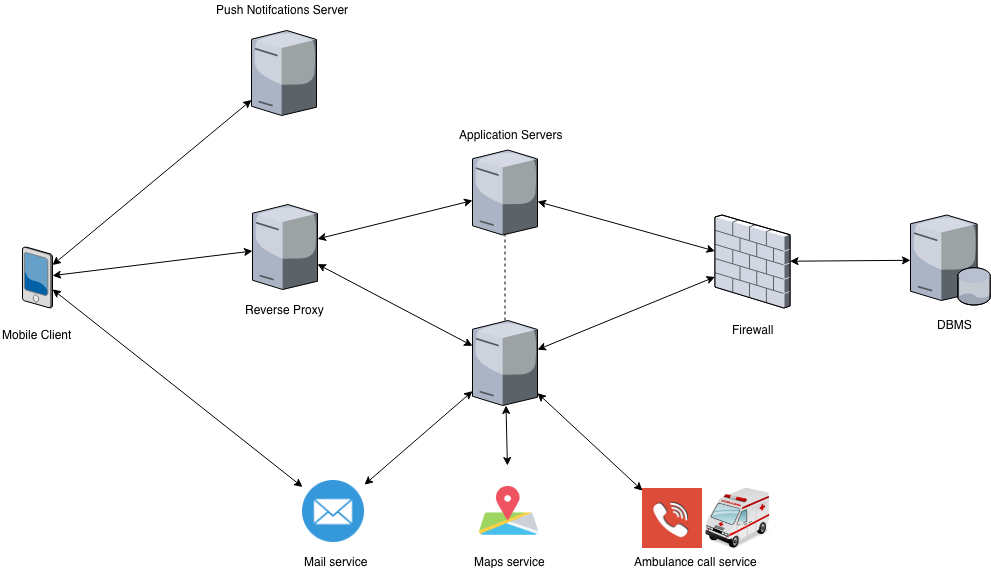
\includegraphics[width=\linewidth]{../images/design/OverviewDiagram.png}
		\end{figure}
		
		\item \textit{\textbf{Component view}}\\\\
		\begin{figure}[H]
		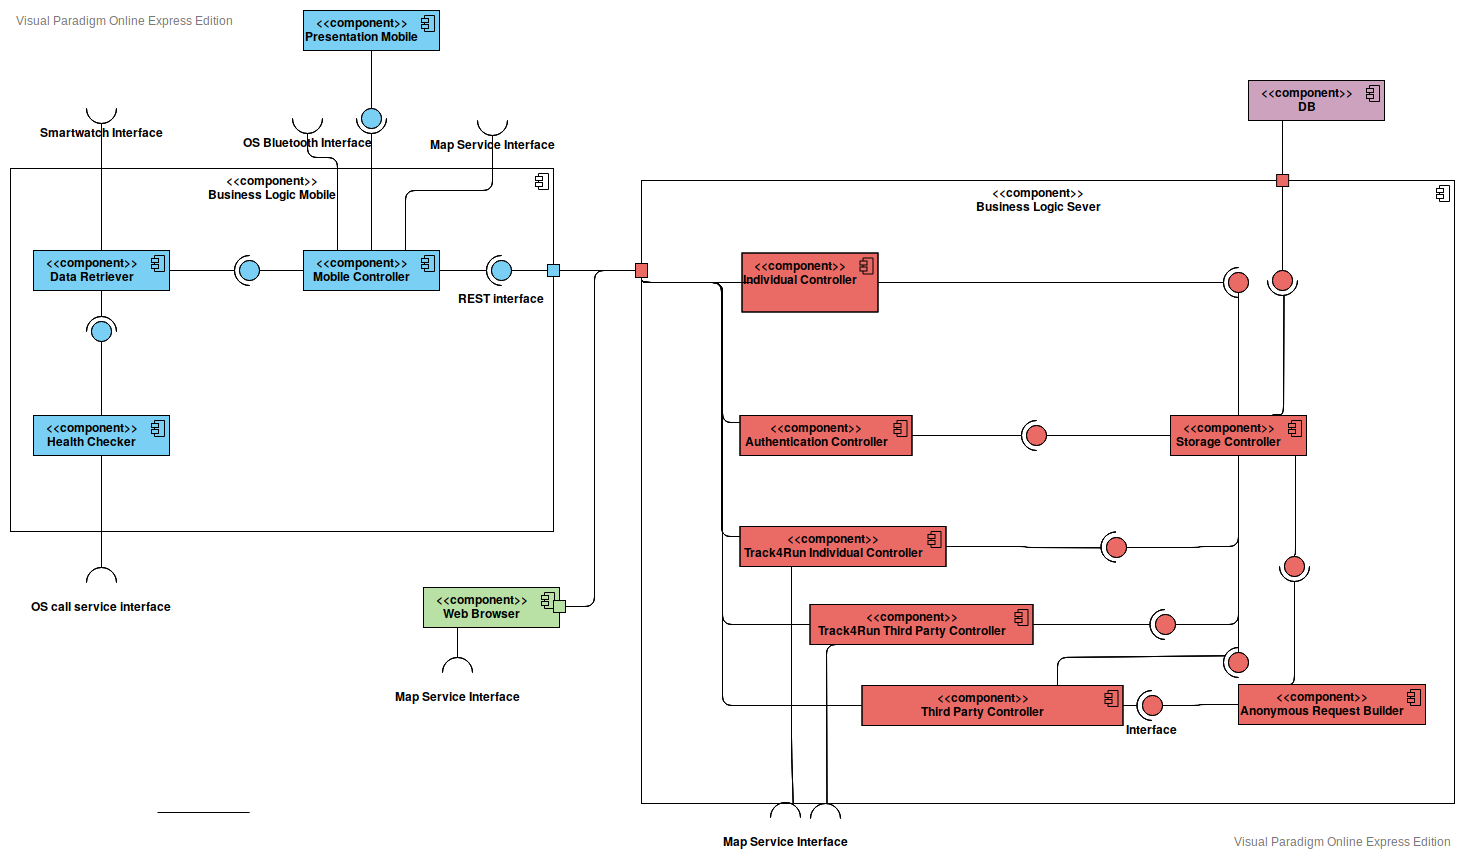
\includegraphics[width=\linewidth]{../images/design/ComponentDiagram.png}
		\end{figure}
		The UML component diagram shows the internal structure of the system highlighting the individual modules and the connections among them. Individual components are wired together by using an assembly connector to connect the required interface of one component with the provided interface of another component. Below is the description of the components:\\
		\begin{itemize}
		\item{\textbf{User mobile client}\\
		This is the component that represents the client machine that accesses to the API of the Business Logic container for the user. ???????????????????????? Da completare in base a come lo vogliamo implementare (dati lato utente o no?)
				}\\
		\item{\textbf{Third party mobile client}\\
		This component represents the client machine that accesses to the API of the Business Logic container for the third party. ????????????????????????????????
				}\\
		\item{\textbf{User controller}\\
		The main role of this component is to manage the transfer of data from the client to the server using the interface provided by the Data component. It also provides methods to accept/refuse a request of agreement and to change login credentials. It can communicate with the Notification controller component to display notifications.
				}\\
		\item{\textbf{Third party controller}\\
		This component is built to manage the transfer of data from the system to the third party using the interface provided by the Data component. It also provides methods to send requests of agreement and requests of data to the system. It can communicate with the Notification controller component to display notifications.
				}\\
		\item{\textbf{Authorization controller}\\
		This component provides authentication and registration processes for both the users and the third parties. It takes the needed data from the Data component and communicates the result of the operations trough the Notification controller.
				}\\
		\item{\textbf{User run controller}\\
		This component provides the methods to permit a user to join, leave, check and watch a run. It communicates with the external service that provides maps trough the Map services interface. Every time a user wants to join a run, it calls the Feasability checker that checks if all the constraints are satisfied. Finally, it can access data of the runs trough the Data component and it can call the Notification controller to send notifications.
				}\\
		\item{\textbf{Third party run controller}\\
		This component provides the methods to allow a third party to organize a run. It communicates with the external service that provides maps trough the Map services interface to allow the third party to select the track for the run.
				}\\				
		\item{\textbf{Notification controller}\\
		This component manages the notifications forwarded by the other components. It only shows notifications inside the application.
				}\\
		\item{\textbf{Health checker}\\
		This component is the core of the service AutomatedSOS. It receives data from the Data component, elaborates them and, if needed, communicates to the Call service interface to send an SOS trough the related external service.
				}\\
		\item{\textbf{Feasability checker}\\
		This component is built to check if a user can actually join a run that is shown trough the Mobile client.
		----------- Serve davvero??????????????????????????????????
				}\\
		\item{\textbf{Data}\\
		The Data component provides the set of Classes corresponding to the tables contained in the Database.
				}\\
		\item{\textbf{Storage interface}
		This component provides the methods for querying the Database.
				}\\
		\item{\textbf{Database}
		This component represent the DBMS. It provides the interfaces to retrieve and store data. In the database there are data about users, third parties and the set of agreements among them. It also contains data about the runs.
				}\\
		\item{\textbf{External services interfaces}\\
      	\begin{itemize}
      	\item{\textbf{Map services interface}\\\
      	It communicates with the map service to allow the third party to select the track and to show the position of runners in real time on the map.
					}\\
			\item{\textbf{Call service interface}\\
			It communicates with the external service to dispatch automatic calls (or emails?) in case of emergency.
					}\\
      	\end{itemize}
				}
		\end{itemize}

		\item \textit{\textbf{Deployment view}}\\\\
		The figure below shows the deployment diagram of the whole system. Its main goal is to describe the distribution of components capturing the topology of the
system's hardware.\\
		\begin{figure}[H]
		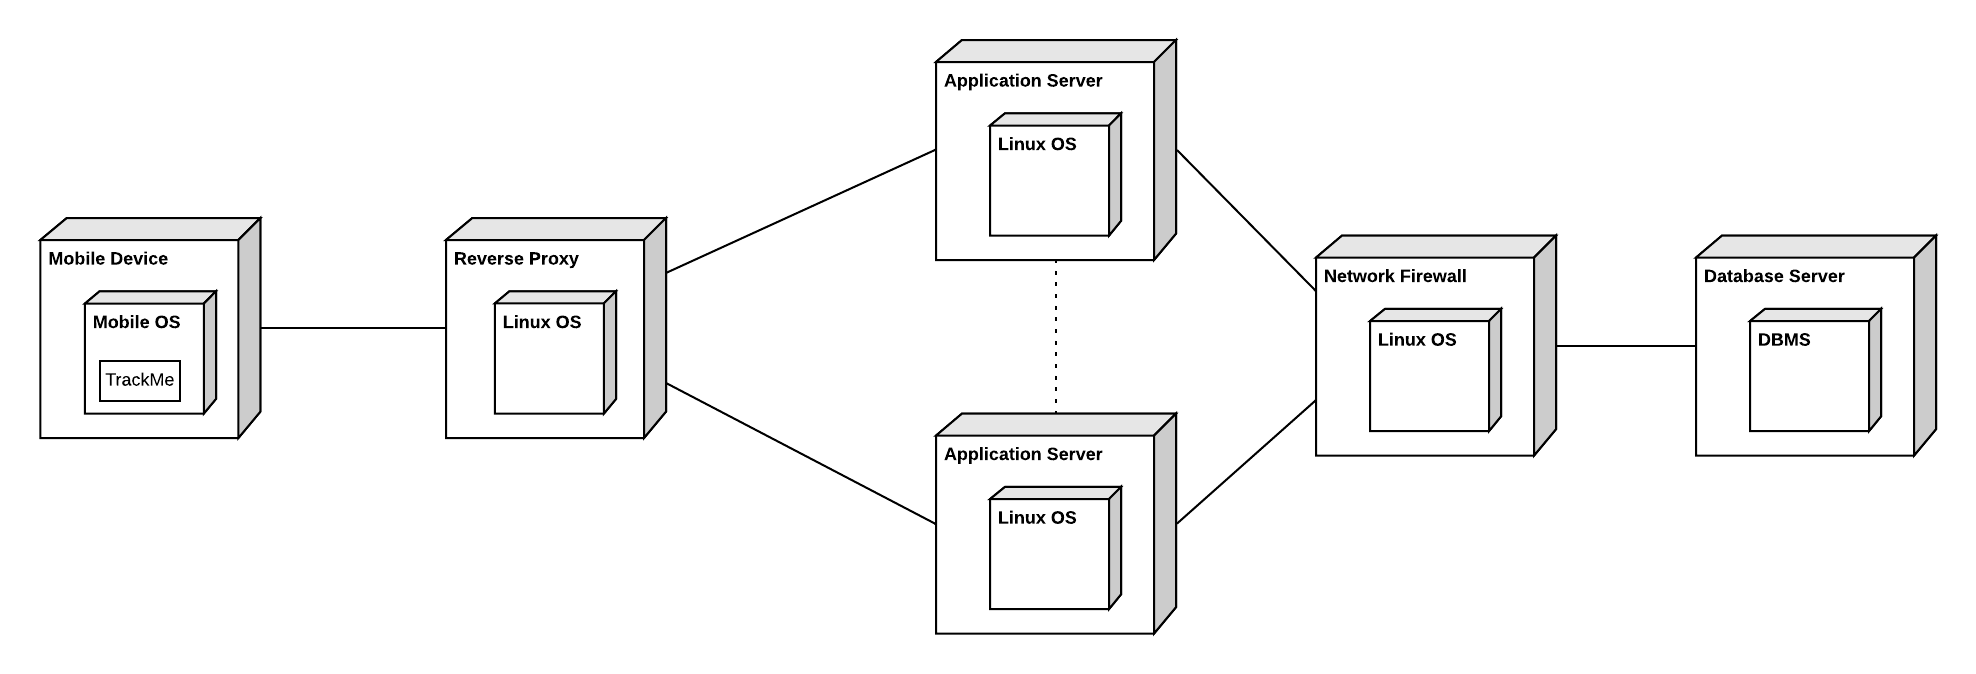
\includegraphics[width=\linewidth]{../images/design/DeploymentDiagram.png}\\
		\end{figure}
		As previously stated in the section 1, the system is structured in a multi-tier architecture. The specific role of each node is clarified here:\\\\
		\textbf{Clients}\\
The first tier is composed by the clients machines (mobile for individuals and desktop for third parties). The individuals will be able to access TrackMe functionalities through the dedicated native application while the third parties through any web browser.\\\\
		\textbf{Application Server}\\
This is the middleware level of the architecture: all the business logic of
the system is contained in this server.\\\\
		\textbf{Network Firewall}\\
The access to the Database is mediated by a network firewall in order to
avoid unauthorised access to the data and the credentials of the user.\\\\
		\textbf{Database Server}\\
This is the last layer of the architecture: all the data are stored in a Database Server accessed through a relational DBMS. \\\\

		\item \textit{\textbf{Runtime view}}\\
			\begin{legal}
				\item \textbf{Sign up Runtime View}\\
				\item \textbf{Login Runtime View}\\
				\item \textbf{Join a run Runtime View}\\
				\item \textbf{Organise a run Runtime View}\\
				\item \textbf{Individual request Runtime View}\\
				\item \textbf{Group request Runtime View}\\
			\end {legal}
		\item \textit{\textbf{Component interfaces}}\\\\
		\item \textit{\textbf{Selected architectural styles and patterns}}\\\\
  	\end{legal}
